\documentclass[../main.tex]{subfiles}

\begin{document}
\section{Programmazione Reattiva}
Con programmazione reattiva si intende un paradigma di programmazione dichiarativo basato sullo stream dei dati e sulla propagazione dei cambiamenti, fortemente correlato con i pattern Observer, Reactor ed il paradigma Event-Driven.\\
Un programma reattivo è costruito definendo la logica della computazione ma non il flusso di controllo, il quale è definito dal verificarsi degli eventi.\\

\subsection{Modelli di valutazione}
Il cambiamento di un valore deve essere propagato automaticamente a tutte le sue dipendenze, azionando la ricomputazione attraverso la notifica. I modi possibili per la propagazione dei cambiamenti e quindi la loro valutazione sono:
\begin{description}
    \item[Push:] (paradigma consumer) I consumatori ricevono dalle sorgenti i dati non appena questi diventano disponibili. 
    \item[Pull:] (paradigma producer) I consumatori richiedono regolarmente i dati ai produttori.
    \item[Push-Pull:] I consumatori ricevono una notifica che descrive il cambiamento e per ottenere le informazioni necessarie devono richiederli ai produttori.
\end{description}
Il modello Push-Pull, chiamato anche backpressure, consiste in una modifica del modello Push che permette ai consumatori di inviare segnali di feedback ai produttori riguardanti l'andamento della propagazione del cambiamento. Il produttore può richiedere (Pull) quanti elementi desidera se questi sono disponibili, ma se questi non sono disponibili vengono ricevuti (Push) non appena lo diventano.\\

\subsection{Observable e Stream}
Con observer si intende l'entità che si sottoscrive ad un observable in modo da essere notificato e reagire ad ogni elemento che esso emette. Mentre gli observable rappresentano quindi degli stream di dati asincroni che possono essere concatenati insieme (dipendenze) per definire in modo dichiarativo nuovi stream più complessi.\\

\begin{figure}[H]
\centering
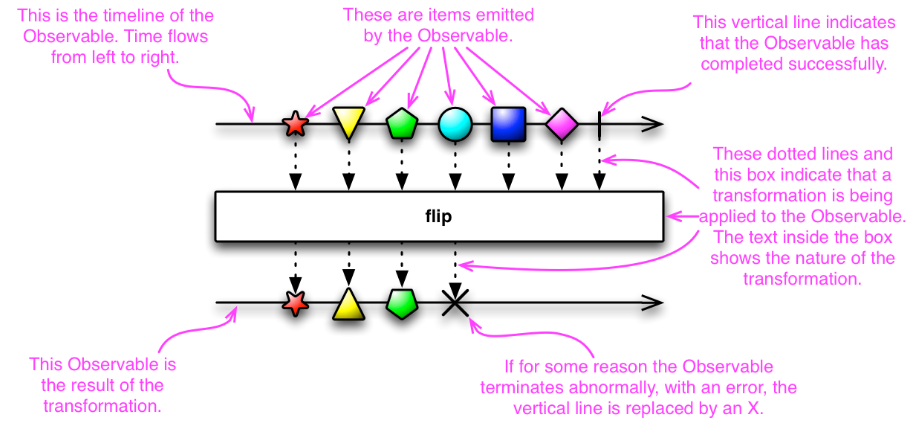
\includegraphics[width=1\textwidth]{img/observable1.png}
\caption{Esempio di Observable - Marble Diagram}
\end{figure}

Le tipologie di stream sono classificate in base a quando l'observable inizia ad emettere i dati:
\begin{description}
    \item[Hot:] L'observable inizia ad emettere dati appena viene creato (modalità eager) e continua senza considerare quanti observer sono registrati. Quando un observer si registra riceve dati solo dal quel momento in poi a meno che non si faccia uso di altri meccanismi come cache/replay.
    \item[Cold:] L'observable inizia ad emettere dati solamente quando si registra almeno un observer (modalità lazy). Ogni volta che un nuovo observer si registra l'observable riiniza ad emettere i dati da capo garantendo gli stessi dati a tutti gli observer.
    \item[Connectable:] L'observable accetta sottoscrizioni dagli observer ma inizia ad emettere dati solamente quando viene invocato l'apposito metodo.
\end{description}

\section{FP + RP}
Il multiparadigma chiamato Functional Reactive Programming (FRP) consiste nella combinazione dei paradigmi funzionale (FP) e reattivo (RP): permette infatti di manipolare stream di dati in modo asincrono con backpressure non-bloccante utilizzando le feature del paradigma funzionale come immutabilità, assenza di side-effects, referential transparency, ...). In RP "\textit{everything is a stream}" mentre in FP "\textit{everything is a function}". \\

I concetti chiave alla base del paradigma FRP sono i due tipi di dato \textit{Behavior} e \textit{Event}, ognuno dei quali con i propri combinatori. Alcuni sistemi FRP non fanno distinzione, modellando entrambi i due tipi di dato con il concetto \textit{Signal}:
\begin{description}
    \item[Behavior] - Modella valori che variano nel tempo. Altri sinonimi di behavior sono \textit{Property} o \textit{Cell}. I behavior modellano lo stato, valori che possono essere ottenuti in qualsiasi momento.
    \item[Event] - Modella un sequenza di eventi in ordine cronologico. Altri sinonimi di event sono \textit{Stream} o \textit{Observable}. Un evento viene propagato attraverso uno stream in un preciso momento, in questo caso si dice che lo stream è attivo (\textit{fired}). Gli stream a differenza dei behavior modellano i cambiamenti dello stato, valori che possono essere ottenuti solamente nell'istante in cui uno stream è attivo.
\end{description}

Un programma FRP è quindi un insieme di behavior e event, costruito partendo da valori statici (che non variano nel tempo) e/o altri behavior/event.

\section{ReactiveStreams}

\end{document}